\begin{frame}
	\myheading{Module 13.2 : Visualizing filters of a CNN
	\textbf{}}
\end{frame}

%%%%%%%%%%%%%%%%%%%%%%%%%%%%%%%%%%%%%%%%%%%%%%%%%%%%%%%%%%%%%%%%%%%%%%%%%%%%%%%%%%%%%%%%%

\begin{frame}
	\begin{columns}
		\column{0.5\textwidth}
		\begin{overlayarea}{\textwidth}{\textheight}
			\only<1-3>{
				\begin{figure}
					\begin{center}
						\tikzstyle{input_neuron}=[circle,draw=red!50,fill=red!10,thick,minimum size=6mm]
\tikzstyle{hidden_neuron}=[circle,draw=blue!50,fill=cyan!10,thick,minimum size=6mm]
\tikzstyle{output_neuron}=[circle,draw=green!50,fill=green!10,thick,minimum size=6mm]
\tikzstyle{cpy_neuron}=[circle,draw=blue!50,fill=blue!50,thick,minimum size=6mm]
\tikzstyle{input}=[circle,draw=black!50,fill=black!20,thick,minimum size=6mm]

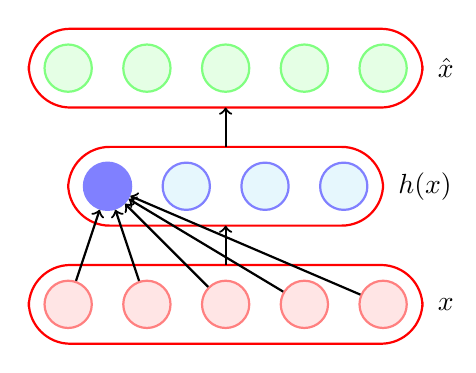
\begin{tikzpicture}

	\node [input_neuron] (neuron01) at (6.5,4.5) {};
	\node [input_neuron] (neuron02) at (7.5,4.5){};
	\node [input_neuron] (neuron03) at (8.5,4.5) {};
	\node [input_neuron] (neuron04) at (9.5,4.5) {};
	\node [input_neuron] (neuron05) at (10.5,4.5) {};
	\node [cpy_neuron] (neuron51) at (7,6) {} ;
	\node [hidden_neuron] (neuron52) at (8,6)  {};
	\node [hidden_neuron] (neuron53) at (9,6)  {};
	\node [hidden_neuron] (neuron54) at (10,6)  {};
	
	\node [output_neuron] (neuron11) at (6.5,7.5)  {};
	\node [output_neuron] (neuron12) at (7.5,7.5)  {};
	\node [output_neuron] (neuron13) at (8.5,7.5)  {};
	\node [output_neuron] (neuron14) at (9.5,7.5)  {};
	\node [output_neuron] (neuron15) at (10.5,7.5)  {};
	
	\node[text width=0.01cm] at (11.2,4.5) {$x$};
	\node[text width=0.01cm] at (10.7,6) {$h(x)$};
	\node[text width=0.01cm] at (11.2,7.5) {$\hat{x}$};
	
	%\node[] at (8.5,3.2) {AE approach};
	
	\draw[red!100,thick,solid,rounded corners=15pt] (6,4) rectangle (11,5);
	\draw[red!100,thick,solid,rounded corners=15pt] (6.5,5.5) rectangle (10.5,6.5);
	\draw[red!100,thick,solid,rounded corners=15pt] (6,7) rectangle (11,8);
	\draw[thick,->](neuron01) -- (neuron51);
	\draw[thick,->](neuron02) -- (neuron51);
	\draw[thick,->](neuron03) -- (neuron51);
	\draw[thick,->](neuron04) -- (neuron51);
	\draw[thick,->](neuron05) -- (neuron51);
	
	\draw[thick,->] (8.5,5) -- (8.5,5.5);
	
	\draw[thick,->] (8.5,6.5) -- (8.5,7);

\end{tikzpicture}

					\end{center}
					%\vspace{-1.5cm}
				\end{figure}
				
			}
			\footnotesize{
				\begin{block}{}
					\begin{align*}
						\underset{x}{\max} \hspace{0.1in} & \{w^Tx\}                        \\
						s.t.\hspace{0.1in}  ||x||^{2}     & = x^{T}x = 1                    \\
						\text{Solution:}\hspace{0.1in}  x & = \frac{w_{1}}{\sqrt{w_1^Tw_1}} 
					\end{align*}
				\end{block}}
		\end{overlayarea}
		\column{0.5\textwidth}
		\begin{overlayarea}{\textwidth}{\textheight}
			\begin{itemize}
				\justifying
				\onslide<1->{\item Recall that we had done something similar while discussing autoencoders}
				\onslide<2->{\item We are interested in finding an input which maximally excites a neuron}
				\onslide<3->{\item Turns out that the input which will maximally activate a neuron is $\frac{W}{\parallel W \parallel}$}
			\end{itemize}
		\end{overlayarea}
	\end{columns}
\end{frame}

%%%%%%%%%%%%%%%%%%%%%%%%%%%%%%%%%%%%%%%%%%%%%%%%%%%%%%%%%%%%%%%%%%%%%%%%%%%%%%%%%%%%%%%%%

\begin{frame}
	\begin{columns}
		\begin{column}{0.5\textwidth}
			\begin{overprint}
				\begin{tikzpicture}[square/.style={regular polygon,regular polygon sides=4}]
	%\begin{axis}[xlabel=x axis label,ylabel=y axis label]
    
	\onslide<1->{
		\foreach \i in {1,...,9}
		{
              
			\pgfmathtruncatemacro{\label}{\i};
			\node[square,draw=red!50,fill=orange!10,thick,minimum size=.2mm] (\label) at (-1*\i*0.5,-3) {};
		}
		\node[square,draw=red!50,fill=orange!10,thick,minimum size=.2mm] (10) at (1,-3) {};
		\path (1) -- node [red, font=\Huge, midway, sloped]{$\dots$} (10);
		%\end{axis}
         
		\draw [
			thick,
			decoration={
				brace,
				mirror,
				raise=0.5cm
			},
			decorate
		] (9) -- (10)
		node [pos=0.5,anchor=south,yshift=-1.1cm] {16};
		%\end{tikzpicture}
         
		%\begin{tikzpicture}[square/.style={regular polygon,regular polygon sides=4}]
		%% Grid 4
		\begin{scope}[scale=2.5,transform shape]
			\node[opacity=0.3] at (-1.17,-2.45) {\Huge{2}};
		\end{scope}
		\draw[step=0.5cm,gray,very thin] (-4,-7) grid (-2,-5);
		\node[] at (-1.5,-6) {*};
         
		\draw[step=0.5cm,gray,very thin] (-1,-6.50) grid (0,-5.5) ;
		\node[] at (0.5,-6) {=};
		%   \node[] at (1,-5.5) {$h_{11}$};
		\node[square,draw=blue!50,fill=blue!10,thick,minimum size=1mm] (1) at (1,-6) {};
     
		%% first row
		\node[circle,fill=\firstrowcolor,inner sep=0pt,minimum size=5.5pt](A) at (-3.75,-5.25   ) {};
		\node[circle,fill=\firstrowcolor,inner sep=0pt,minimum size=5.5pt](B) at (-3.75+0.5,-5.25   ) {};
     
		\node[circle,fill=\secondrowcolor,inner sep=0pt,minimum size=5.5pt](C) at (-3.75+2*0.5,-5.25    ) {};
		\node[circle,fill=\secondrowcolor,inner sep=0pt,minimum size=5.5pt](D) at (-3.75+3*0.5,-5.25    ) {};
     
		%% second row
		\node[circle,fill=\firstrowcolor,inner sep=0pt,minimum size=5.5pt](F) at (-3.75+0.5,-5.25-0.5   ) {};
		\node[circle,fill=\firstrowcolor,inner sep=0pt,minimum size=5.5pt](E) at (-3.75,-5.25-0.5   ) {};
		\node[circle,fill=\secondrowcolor,inner sep=0pt,minimum size=5.5pt](G) at (-3.75+2*0.5,-5.25-0.5    ) {};
		\node[circle,fill=\secondrowcolor,inner sep=0pt,minimum size=5.5pt](H) at (-3.75+3*0.5,-5.25-0.5    ) {};
     
		%% 3rd row
		\node[circle,fill=\thirdrowcolor,inner sep=0pt,minimum size=5.5pt](J) at (-3.75+0.5,-5.25-2*0.5 ) {};
		\node[circle,fill=\thirdrowcolor,inner sep=0pt,minimum size=5.5pt](I) at (-3.75,-5.25-2*0.5 ) {};
		\node[circle,fill=\fourrowcolor,inner sep=0pt,minimum size=5.5pt](K) at (-3.75+2*0.5,-5.25-2*0.5    ) {};
		\node[circle,fill=\fourrowcolor,inner sep=0pt,minimum size=5.5pt](L) at (-3.75+3*0.5,-5.25-2*0.5    ) {};
     
		%% 4th row
     
		\node[circle,fill=\thirdrowcolor,inner sep=0pt,minimum size=5.5pt](N) at (-3.75+0.5,-5.25-3*0.5 ) {};
		\node[circle,fill=\thirdrowcolor,inner sep=0pt,minimum size=5.5pt](M) at (-3.75,-5.25-3*0.5 ) {};
		\node[circle,fill=\fourrowcolor,inner sep=0pt,minimum size=5.5pt](O) at (-3.75+3*0.5,-5.25-3*0.5    ) {};
		\node[circle,fill=\fourrowcolor,inner sep=0pt,minimum size=5.5pt](P) at (-3.75+2*0.5,-5.25-3*0.5    ) {};
     
     
		\node[circle,fill=blue,inner sep=0pt,minimum size=5.5pt](Ai) at (-0.75,-5.75    ) {};
     
		\node[circle,fill=blue,inner sep=0pt,minimum size=5.5pt](Bi) at (-0.75+0.5,-5.75    ) {};
     
		\node[circle,fill=blue,inner sep=0pt,minimum size=5.5pt](Bi) at (-0.75,-5.75-0.5    ) {};
     
		\node[circle,fill=blue,inner sep=0pt,minimum size=5.5pt](Bi) at (-0.75+0.5,-5.75-0.5    ) {};
     
	}




	
	\onslide<1->{
		\node[square,draw=blue!50,fill=blue!10,thick,minimum size=1mm] (11) at (-3.25,-1.5) {};
     
		\foreach \i in {9,8,5,4}
		{
			\draw [-,draw=black!50] (\i) -- (11);
		}
		\node[] at (-3.25,-1.1) {$h_{11}$};
     
     
	}


	\onslide<1->{
		\node[] at (-2.25,-1.1) {$h_{12}$};
		\node[square,draw=blue!50,fill=blue!10,thick,minimum size=1mm] (12) at (-2.25,-1.5) {};
		\foreach \i in {7,6,3,2}
		{
			\draw [-,draw=black!50] (\i) -- (12);
		}
	}


	\only<1->{
     
		\renewcommand{\firstrowcolor}{black}
		\renewcommand{\secondrowcolor}{black}
		\renewcommand{\thirdrowcolor}{black}
		\renewcommand{\fourrowcolor}{red}
     
     
		\node[circle,fill=\fourrowcolor,inner sep=0pt,minimum size=5.5pt](O) at (-3.75+3*0.5,-5.25-3*0.5    ) {};
		\node[circle,fill=\fourrowcolor,inner sep=0pt,minimum size=5.5pt](P) at (-3.75+2*0.5,-5.25-3*0.5    ) {};
     
		\node[circle,fill=\fourrowcolor,inner sep=0pt,minimum size=5.5pt](K) at (-3.75+2*0.5,-5.25-2*0.5    ) {};
		\node[circle,fill=\fourrowcolor,inner sep=0pt,minimum size=5.5pt](L) at (-3.75+3*0.5,-5.25-2*0.5    ) {};
		\node[circle,fill=blue,inner sep=0pt,minimum size=5.5pt](Ai) at (-0.75,-5.75    ) {};
     
		\node[circle,fill=blue,inner sep=0pt,minimum size=5.5pt](Bi) at (-0.75+0.5,-5.75    ) {};
     
		\node[circle,fill=blue,inner sep=0pt,minimum size=5.5pt](Bi) at (-0.75,-5.75-0.5    ) {};
     
		\node[circle,fill=blue,inner sep=0pt,minimum size=5.5pt](Bi) at (-0.75+0.5,-5.75-0.5    ) {};
     
		\node[] at (1,-5.5) {$h_{14}$};
	}
	%% Grid 2

\end{tikzpicture}
			\end{overprint}
			       
		\end{column}
		\begin{column}{0.5\textwidth}
			\begin{itemize}
				\justifying
				\setlength\itemsep{1em}
				\item<1-> Now recall that we can think of a CNN also as a feed-forward network with sparse connections and weight sharing
				\item<2-> Once again, we are interested in knowing what kind of inputs will cause a given neuron to fire 
				\item<3-> The solution would be the same $(\frac{W}{\parallel W \parallel})$ where $W$ is the filter($2\times 2$, in this case)
				\item<4-> We can thus think of these filters as pattern detectors
			\end{itemize}
		\end{column}
		   
	\end{columns}
\end{frame}

%%%%%%%%%%%%%%%%%%%%%%%%%%%%%%%%%%%%%%%%%%%%%%%%%%%%%%%%%%%%%%%%%%%%%%%%%%%%%%%%%%%%%%%%%

\begin{frame}
	\begin{columns}
		\column{0.5\textwidth}
		\begin{overlayarea}{\textwidth}{\textheight}
			\begin{figure}
				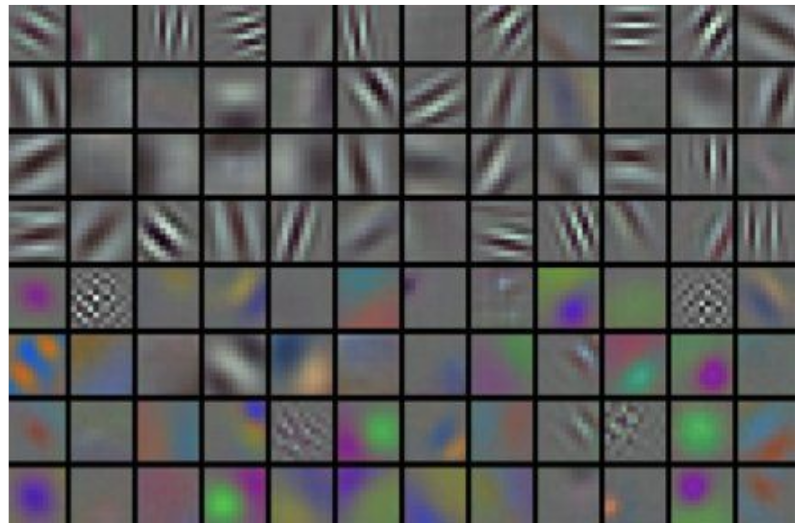
\includegraphics[scale=0.15]{images/kfilter.png}
			\end{figure}
			\footnotesize{
				\begin{block}{}
					\begin{align*}
						\underset{x}{\max} \hspace{0.1in} & \{w^Tx\}                        \\
						s.t.\hspace{0.1in}  ||x||^{2}     & = x^{T}x = 1                    \\
						\text{Solution:}\hspace{0.1in}  x & = \frac{w_{1}}{\sqrt{w_1^Tw_1}} 
					\end{align*}
				\end{block}
			}
		\end{overlayarea}
		\column{0.5\textwidth}
		\begin{overlayarea}{\textwidth}{\textheight}
			\begin{itemize}
				\justifying
				\onslide<1->{\item We can simply plot the $K \times K$ weights (filters) as images \& visualize them as patterns}
				\onslide<2->{\item The filters essentially detect these patterns (by causing the neurons to maximally fire)}
				\onslide<3->{\item This is only interpretable for the filters in the first convolution layer \onslide<4->{(Why?)}}
			\end{itemize}
		\end{overlayarea}
	\end{columns}
\end{frame}